% English version of paper/ja_v2/06_問い2.md (2026-11-17).
\section{RQ2: combining predictions with strengths from the K labels and per-emotion profiles from the sources had higher UAR than the product in 11 of 12 conditions}\label{sec:rq2}

RQ2 asks how the predictions of the audio, visual and text classifiers should be combined into pseudo-labels. Late fusion with reliabilities whose strengths are measured on the K target labels and whose per-emotion profiles are measured on the source corpora (the proposal) had higher UAR than the equal-weight product of the three probabilities in 11 of 12 conditions on AFEW, IEMOCAP (improvised), MOSEI and MELD in point estimates, by 2.1--3.5\pt\ on AFEW. Differences from methods that tune temperatures or weights on the K labels varied in sign across conditions. The proposal was higher than selecting the single strongest classifier on the K labels in all 12 conditions in point estimates.

\subsection{Setting}

\subsubsection{Idea: the strongest modality differs by corpus and emotion}\label{sec:idea}
The product used in Sect.~\ref{sec:rq1b} multiplies the three probabilities with equal weights, but which modality recognises each emotion best differed by corpus and emotion (Fig.~\ref{fig:idea}). In provisional-target computations run to design the method (Sect.~\ref{sec:settings}; each of the four corpora as a provisional target with two of the remaining corpora as sources, 30 repetitions each), the classifier-by-emotion reliabilities (Sect.~\ref{sec:method}) measured with all candidate labels were highest for visual on all four emotions of AFEW and for text on all four of MELD, for visual on Happy and audio on the others in IEMOCAP, and changed with the emotion in MOSEI. The equal-weight product does not use these differences. In the AFEW evaluation run, for example, the visual classifier of the product had a UAR more than 17\pt\ above the audio and text classifiers (K = 5: visual 70.70, audio 53.24, text 45.76), and the visual classifier alone was higher than the product at K = 5 and 10 in point estimates (70.70 vs 69.23 and 71.93 vs 70.88). Section~\ref{sec:rq1b} showed that the gain of distillation ranked with the advantage of the pseudo-labels, so the proposal changes the classifier-by-emotion weights per target corpus to raise the UAR of the pseudo-labels.

\begin{figure}[t]
\centering
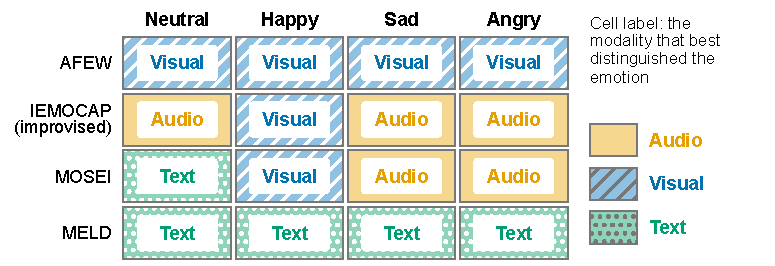
\includegraphics[width=\textwidth]{figures/fig_prop_idea_en.pdf}
\caption{For each corpus and emotion, the modality with the highest reliability. Values are reliabilities used to design the method (provisional-target computations, all candidate labels, K = 5, mean of 30 repetitions), not values of the evaluation run}\label{fig:idea}
\end{figure}

Measuring all 12 weights on the K target labels would determine each weight from only K utterances per emotion. The same computations showed that the weights can be split into two parts that can be measured differently. We built two classifier-by-emotion reliability tables, one measured on the sources and one on all candidate labels of the provisional target (ranges below are minima and maxima over four corpora $\times$ K = 5, 10, 25). First, the ranking of classifier strengths (mean reliability over the four emotions) changed across corpora and could not be measured on the sources: the correlation between the strengths in the two tables was $-$0.954 to +0.403, and the strongest modality agreed between the two in 0--0.467 of repetitions (0.433--1.000 for strengths measured on the K labels). Second, the classifier-by-emotion component left after fitting classifier and emotion effects and Tukey's one-degree-of-freedom non-additivity term \cite{tukey1949} correlated 0.463--0.780 between the two tables and could be measured on the sources. The proposal therefore measures strengths on the K target labels and per-emotion profiles on the labelled source corpora.

\subsubsection{Method: emotion-wise reliability-weighted late fusion}\label{sec:method}
The proposal weights the predictions of the classifiers that make the product in Sect.~\ref{sec:rq1b} (the product components) with a classifier-by-emotion reliability table and turns the fused predictions into pseudo-labels. The table is the sum of strengths and per-emotion profiles (Fig.~\ref{fig:decomp}).

\begin{figure}[t]
\centering
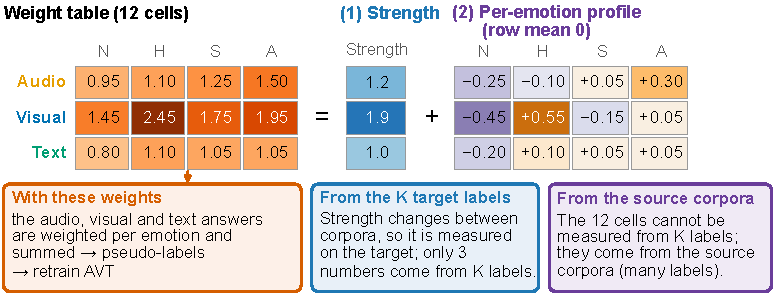
\includegraphics[width=\textwidth]{figures/fig_prop_decomp_en.pdf}
\caption{The 12-cell classifier-by-emotion weight table split into (1) one strength per classifier, measured on the K target labels (three numbers), and (2) per-emotion profiles, measured on the source corpora (each row sums to zero). Numbers are illustrative}\label{fig:decomp}
\end{figure}

The reliability is defined on the scores of each classifier. With probabilities $p_m(i\mid x)$ of classifier $m$ for emotion $i$, the centred log-probability is the score $z_m(i\mid x)=\log p_m(i\mid x)-\frac14\sum_j\log p_m(j\mid x)$, and
\begin{equation}\label{eq:rel}
d_m(i)=\max\!\big(0,\sqrt2\,\Phi^{-1}(A_m(i))\big),\quad A_m(i)\in[0.02,0.98],
\end{equation}
where $A_m(i)$ is the mean over emotions $j\neq i$ of the area under the ROC curve (AUC) separating utterances of true emotion $i$ from those of $j$ by $z_m(i\mid\cdot)$, and $\Phi^{-1}$ is the standard normal quantile function ($d_m(i)\le 2.90$). Because the ranks of scores do not change when intercepts are shifted, $d_m(i)$ depends neither on the classifier's intercepts nor on the target's emotion proportions. The mean over the four emotions is the strength $L_m$, and $d_m(i)-L_m$ is the per-emotion profile.

The strengths are measured on the K labels. The K labels are split into five subsets per emotion; for each subset $f$, the product components are retrained by the procedure of Sect.~\ref{sec:rq1b} on the K labels without subset $f$ and assign probabilities to subset $f$; the reliabilities of Eq.~(\ref{eq:rel}) computed from the five subsets' probabilities are averaged over emotions to give $L^{K}_m$ (Fig.~\ref{fig:calc}a). Because $L^{K}_m$ is noisy for small K, a default strength $L^{0}_m$ (the mean of the three $L^{K}_m$ or the strength measured on the sources) is mixed in with weight $n_0$:
\begin{equation}
L_m=\frac{n\,L^{K}_m+n_0\,L^{0}_m}{n+n_0},\qquad n=4K.
\end{equation}

The profiles are measured on the source corpora. Within each source $s$, $d^{\mathrm{in}}_{s,m}(i)$ is measured by speaker-split five-fold cross-validation, and a classifier trained on all of $s$ is applied to another source $t$ to give $d^{\mathrm{out}}_{s\to t,m}(i)$. The share of modality $m$'s reliability that carries over to other corpora is $\eta_m=\sum_{s\to t}\sum_i d^{\mathrm{out}}_{s\to t,m}(i)/\sum_{s\to t}\sum_i d^{\mathrm{in}}_{s,m}(i)$ (clipped to $[0,1.5]$), and
\begin{equation}
d^{\mathrm{src}}_m(i)=\eta_m\frac{1}{|S|}\sum_s d^{\mathrm{in}}_{s,m}(i),\qquad r^{\mathrm{src}}_m(i)=d^{\mathrm{src}}_m(i)-\frac14\sum_j d^{\mathrm{src}}_m(j)
\end{equation}
(Fig.~\ref{fig:calc}b).

\begin{figure}[t]
\centering
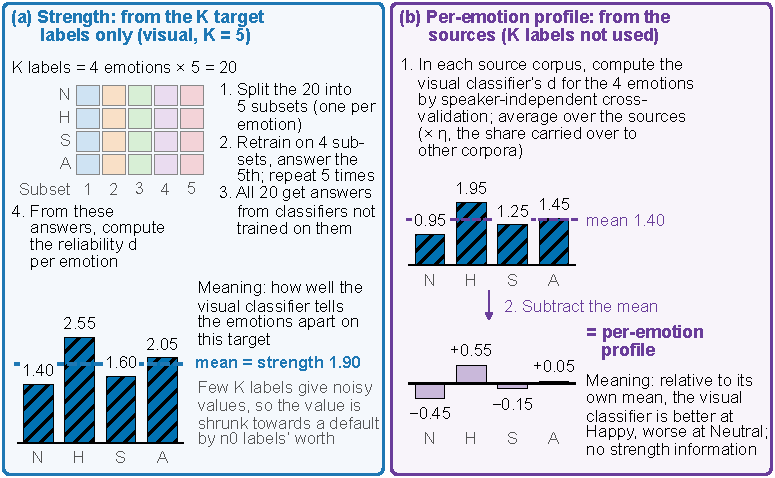
\includegraphics[width=\textwidth]{figures/fig_prop_calc_en.pdf}
\caption{Computing the strength and the per-emotion profile (visual classifier, K = 5). (a) The 20 K labels are split into five subsets, the classifier retrained on four subsets labels the fifth, repeated five times; the per-emotion reliabilities $d$ of these predictions are averaged into the strength. (b) Reliabilities from cross-validation within the source corpora minus their mean over emotions give the profile. Numbers are illustrative}\label{fig:calc}
\end{figure}

The reliability table combines strengths and profiles, and the fused predictions give the pseudo-labels. The table is $T(m,i)=\max(0,L_m+\beta\,r^{\mathrm{src}}_m(i))$ ($\beta=1$ uses the profiles, $\beta=0$ does not); dividing by its mean gives weights $\Omega(m,i)=T(m,i)/(\frac{1}{12}\sum_{m',i'}T(m',i'))$, and the scores are summed per emotion, $s(i\mid x)=\sum_m \Omega(m,i)\,z_m(i\mid x)$. Because emotion-specific weights can shift predictions towards some emotions, intercepts $c$ are shifted without labels so that the mean of $\mathrm{softmax}(s(\cdot\mid x)+c)$ over candidates equals the mean of the product's probabilities (fixed-point iteration). The fused decision at estimation time is $\arg\max_i(s(i\mid x)+c_i)$. We attach $q(i\mid x)=\mathrm{softmax}_i(s(i\mid x)+c_i)$ to the candidates as pseudo-labels (soft labels) and retrain the AVT classifier (AV for CREMA-D) with the loss of Sect.~\ref{sec:rq1b}. Because the fused predictions carry information of all three modalities, the retrained classifier is AVT, which takes all three features; comparisons of estimation-time decisions (set A in Sect.~\ref{sec:compare}) do not depend on it. Audio, visual and text classifiers retrained on the proposal's pseudo-labels were not computed (Sect.~\ref{sec:limitations}). $\rho$ and $a$ are borrowed from the values chosen for the product's pseudo-labels.

\subsubsection{Hyperparameter selection on source-corpus episodes}\label{sec:hp}
The hyperparameters ($n_0\in\{0,20,80,\infty\}$, $\beta\in\{0,1\}$ and the two default strengths; 16 settings, 14 distinct) were selected, per evaluation target and K, by the highest mean UAR on the test folds of the provisional targets over three episodes in which each source corpus served in turn as a provisional target with the other two as sources (3 corpora $\times$ 5 folds $\times$ 2 seeds = 30 repetitions; Fig.~\ref{fig:episode}). No data of the evaluation target enter any episode. All selected settings had $\beta=1$, and $n_0$ was 0 in 8 of 12 conditions and 20 in the other four. The setting $n_0=\infty$, $\beta=0$ with the mean default strength gives the same decisions as the product. For CREMA-D, the hyperparameters ($n_0=0$, $\beta=1$) and $\rho$ and $a$ for the AV classifier were selected on the repetitions of a six-corpus provisional-target computation (the four corpora plus CREMA-D and RAVDESS) that do not involve CREMA-D. The form of the method was fixed after seeing the provisional-target runs, and the evaluation was computed once; the idea of the proposal was conceived after seeing outputs of the evaluation run of Sect.~\ref{sec:rq1b}, and CREMA-D was added to the evaluation after its values had been seen in the six-corpus provisional runs (Sect.~\ref{sec:limitations}).

\begin{figure}[t]
\centering
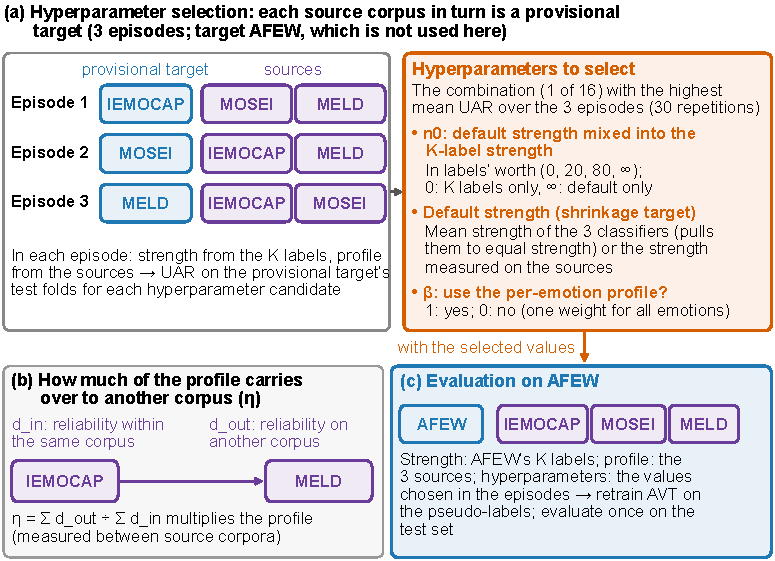
\includegraphics[width=\textwidth]{figures/fig_prop_episode_en.pdf}
\caption{Hyperparameter selection (target AFEW). In three episodes, each source corpus serves as a provisional target; strengths are measured on its K labels and profiles on the other two sources, and the hyperparameter setting with the highest mean UAR on the provisional targets' test folds is chosen. The carry-over $\eta$ of the profiles is measured between sources. AFEW is then evaluated once with the selected values}\label{fig:episode}
\end{figure}

\subsubsection{Evaluation and comparisons}\label{sec:compare}
The evaluation targets are AFEW, IEMOCAP (improvised), MOSEI and MELD, with K = 5, 10 and 25 and 50 repetitions (5 folds $\times$ 10 draws). K labels, candidates, test utterances and product components are those of Sect.~\ref{sec:rq1b}; only the classifiers measuring strengths and the AVT retrained on the proposal's pseudo-labels are new. CREMA-D (audio and visual) is also evaluated with 50 repetitions and four source corpora. The proposal needs K labels, so there is no K = 0 condition. Intervals are those of the LOCO setting (Sect.~\ref{sec:setup}).

Table~\ref{tab:comparators} lists the comparisons. Set A uses the same product components and K labels and differs only in how predictions are combined; it is compared with the proposal's estimation-time decisions. Set B consists of AVT classifiers compared with the AVT retrained on the proposal's pseudo-labels. ``Strongest single classifier'' was added after the evaluation run from its saved outputs (outside the evaluation protocol): the product component with the highest strength measured on the K labels is selected and its predictions are used, with the same label-free intercept shift as the proposal. Four further combinations of the same predictions were also compared (Appendix~\ref{app:extra}).

\begin{table}[t]
\caption{Comparisons. ``From K'' is the number of quantities fitted or selected on the K target labels (the proposal: three strengths)}\label{tab:comparators}
\footnotesize\setlength{\tabcolsep}{4pt}
\begin{tabular}{@{}lp{2.8cm}p{4.0cm}p{2.5cm}l@{}}
\toprule
Set & Comparison & Content & Reference & From K \\
\midrule
A & Product & Multiply the three probabilities with equal weights & Product rule \cite{kittler1998} & 0 \\
A & Mean of probabilities & Average the three probabilities & Sum rule \cite{kittler1998} & 0 \\
A & Strength-only weights & Sum scores with weights proportional to the K-label strengths, common to emotions & Classifier weights \cite{kuncheva2014} & 3 \\
A & Full table from K & All 12 reliabilities measured on the K labels, combined as the proposal & Same number of per-class parameters as a recall combiner \cite{kuncheva2014} & 12 \\
A & Temperature calibration & Per-classifier inverse temperatures fitted to the K-label log-likelihood, then multiplied & Temperature scaling \cite{guo2017calibration} & 3 \\
A & Weight-table search & Among 1,000 random tables and the equal table, the one with the highest K-label UAR & Random search as in Kaya et al.\ \cite{kaya2017} & 1 of 1,001 \\
A & Strongest single classifier & Predictions of the product component with the highest K-label strength & Added in this study & 1 of 3 \\
B & K-label baseline (AVT) & Retrain on the K labels without pseudo-labels & Sect.~\ref{sec:settings} & --- \\
B & Distillation (product) & Retrain AVT on the product's pseudo-labels & Sect.~\ref{sec:rq1b} & --- \\
\botrule
\end{tabular}
\end{table}

\subsection{Results}\label{sec:rq2-results}

\subsubsection{The proposal had higher UAR than the product in 11 of 12 conditions}
Table~\ref{tab:rq2} shows that the estimation-time proposal $-$ product was positive in 11 of 12 conditions on the four corpora other than CREMA-D, with intervals excluding zero in seven (AFEW at all K, IEMOCAP and MOSEI at K = 25, MELD at K = 10 and 25). The largest differences were on AFEW: +2.13 [+1.0, +3.3] (71.36 vs 69.23), +3.51 [+1.5, +5.5] (74.39 vs 70.88) and +3.14 [+1.9, +4.4] (76.58 vs 73.45)\pt\ for K = 5, 10 and 25; the other nine conditions ranged from $-$0.09 to +0.83\pt. The AVT retrained on the proposal's pseudo-labels minus distillation (product) was also positive in 11 of 12 conditions, +1.01, +1.95 and +1.21\pt\ on AFEW (all intervals excluding zero) and $-$0.05 to +0.82\pt\ elsewhere. On CREMA-D (audio and visual), both differences were +0.31 to +0.63\pt\ with all six intervals excluding zero.

Differences from methods that tune temperatures or weights on the K labels varied in sign. Against per-classifier temperature calibration, the proposal was higher in 8 of 12 conditions in point estimates and lower with an interval excluding zero only on AFEW at K = 5 ($-$2.94 [$-$5.6, $-$0.3], 71.36 vs 74.30). Against strength-only weights the differences were $-$1.16 to +0.73\pt, with intervals above zero on MOSEI at all K (+0.51 to +0.73\pt) and on IEMOCAP at K = 5 (+0.24\pt). Against the four further combinations in Appendix~\ref{app:extra}, the proposal was higher in 39 of 48 conditions in point estimates, with intervals above zero in 25 and below zero in none.

Against the strongest single classifier, the proposal was higher in all 12 conditions in point estimates (+2.70 to +5.52\pt), with intervals above zero in seven (IEMOCAP at K = 5, MOSEI and MELD at all K); intervals included zero on AFEW at all K and IEMOCAP at K = 10 and 25 (AFEW interval widths 10.61--12.01\pt). On IEMOCAP, MOSEI and MELD, the product was also higher than this comparison in point estimates (+2.04 to +5.02\pt; intervals above zero in 7 of 9), so most of the difference between the proposal and this comparison came from product $-$ strongest single; on AFEW, product $-$ strongest single was only +0.57 to +0.67\pt\ and most of the difference came from proposal $-$ product. The strongest-single comparison had lower UAR on AFEW at K = 5 (68.65) than the visual classifier alone in Sect.~\ref{sec:idea} (70.70) because a non-visual classifier was selected in 3 of 50 repetitions and the intercepts were shifted (69.25 before shifting). The intercept shift lowered this comparison's UAR on AFEW by 0.44--0.65\pt; without the shift for either method, proposal $-$ strongest single was +1.86 to +6.11\pt\ in all 12 conditions, with intervals above zero in eight. Per emotion, the recall differences proposal $-$ strongest single were negative in point estimates for Happy on AFEW ($-$6.42 to $-$4.39\pt), Neutral on MELD ($-$4.32 to $-$2.74\pt) and Sad on IEMOCAP at K = 25 ($-$0.21\pt); intervals of per-emotion differences were not computed.

\begin{table}[p]
\caption{UAR (points, test utterances, mean of 50 repetitions). For each target, the rows from ``Product'' to ``Strongest single'' are set A and are compared with the estimation-time proposal (est.); the last two rows are set B and are compared with the retrained proposal (retr.; AVT, or AV for CREMA-D). Row names abbreviate those of Table~\ref{tab:comparators} (probs.: probabilities; Strength only: strength-only weights; Full table (K): full table from K; Temperature: temperature calibration; Table search: weight-table search; base.: baseline; Distill.\ (prod.): distillation on the product's pseudo-labels). Parentheses: proposal $-$ row with 95\% intervals without correction. * interval above zero (proposal higher); $\dagger$ below zero (proposal lower). ``Strongest single'' was added after the evaluation and not computed for CREMA-D. Intervals of the weight-table search are conditional on the drawn tables. Strength-only weights gave the same UAR as the proposal without profiles (Table~\ref{tab:ablation}) in 8 of the 12 conditions on the four corpora and in all three on CREMA-D}\label{tab:rq2}
\footnotesize\setlength{\tabcolsep}{2pt}
\begin{tabular}{@{}llll@{}}
\toprule
Row & K = 5 & K = 10 & K = 25 \\
\midrule
\multicolumn{4}{@{}l}{\textbf{AFEW}} \\
Proposal (est.) & 71.36 & 74.39 & 76.58 \\
Product & 69.23 (+2.13 [+1.0, +3.3]*) & 70.88 (+3.51 [+1.5, +5.5]*) & 73.45 (+3.14 [+1.9, +4.4]*) \\
Mean of probs. & 69.22 (+2.14 [+1.0, +3.2]*) & 71.02 (+3.38 [+1.9, +4.9]*) & 72.85 (+3.73 [+2.5, +5.0]*) \\
Strength only & 72.51 ($-$1.16 [$-$2.6, +0.3]) & 73.94 (+0.45 [$-$0.1, +1.0]) & 76.55 (+0.03 [$-$0.5, +0.6]) \\
Full table (K) & 72.55 ($-$1.19 [$-$2.8, +0.4]) & 74.34 (+0.05 [$-$0.6, +0.7]) & 76.84 ($-$0.26 [$-$0.8, +0.3]) \\
Temperature & 74.30 ($-$2.94 [$-$5.6, $-$0.3]$\dagger$) & 74.84 ($-$0.45 [$-$1.5, +0.6]) & 76.31 (+0.27 [$-$0.6, +1.1]) \\
Table search & 71.50 ($-$0.14 [$-$2.4, +2.1]) & 73.80 (+0.59 [$-$1.2, +2.3]) & 76.55 (+0.03 [$-$1.9, +1.9]) \\
Strongest single & 68.65 (+2.70 [$-$3.3, +8.7]) & 70.21 (+4.18 [$-$1.2, +9.6]) & 72.79 (+3.79 [$-$1.5, +9.1]) \\
Proposal (retr.) & 71.78 & 74.61 & 77.05 \\
K-label base. & 69.74 (+2.04 [+0.5, +3.6]*) & 71.56 (+3.05 [+1.8, +4.3]*) & 75.22 (+1.83 [+0.9, +2.8]*) \\
Distill. (prod.) & 70.77 (+1.01 [+0.2, +1.8]*) & 72.66 (+1.95 [+0.5, +3.4]*) & 75.84 (+1.21 [+0.4, +2.0]*) \\
\midrule
\multicolumn{4}{@{}l}{\textbf{IEMOCAP (improvised)}} \\
Proposal (est.) & 72.56 & 73.80 & 75.03 \\
Product & 72.07 (+0.49 [$-$0.2, +1.2]) & 73.37 (+0.43 [$-$0.2, +1.1]) & 74.53 (+0.50 [+0.01, +1.0]*) \\
Mean of probs. & 73.03 ($-$0.46 [$-$2.8, +1.9]) & 74.25 ($-$0.46 [$-$3.1, +2.2]) & 75.52 ($-$0.49 [$-$3.2, +2.2]) \\
Strength only & 72.32 (+0.24 [+0.03, +0.5]*) & 73.57 (+0.23 [$-$0.05, +0.5]) & 74.83 (+0.20 [$-$0.1, +0.5]) \\
Full table (K) & 72.36 (+0.20 [$-$1.7, +2.1]) & 73.75 (+0.05 [$-$0.7, +0.8]) & 75.30 ($-$0.27 [$-$1.1, +0.5]) \\
Temperature & 71.69 (+0.87 [+0.5, +1.2]*) & 73.16 (+0.64 [$-$0.1, +1.4]) & 74.37 (+0.67 [$-$0.2, +1.6]) \\
Table search & 70.41 (+2.15 [+0.9, +3.4]*) & 71.30 (+2.50 [+1.7, +3.3]*) & 73.49 (+1.54 [+1.2, +1.9]*) \\
Strongest single & 67.05 (+5.52 [+1.3, +9.8]*) & 68.42 (+5.38 [$-$0.5, +11.2]) & 71.51 (+3.52 [$-$3.6, +10.7]) \\
Proposal (retr.) & 72.81 & 73.86 & 74.95 \\
K-label base. & 72.55 (+0.25 [$-$4.5, +5.0]) & 73.49 (+0.36 [$-$3.7, +4.4]) & 75.51 ($-$0.56 [$-$4.7, +3.6]) \\
Distill. (prod.) & 72.71 (+0.10 [$-$0.6, +0.8]) & 73.73 (+0.13 [$-$0.3, +0.6]) & 74.68 (+0.27 [$-$0.1, +0.6]) \\
\midrule
\multicolumn{4}{@{}l}{\textbf{MOSEI}} \\
Proposal (est.) & 41.16 & 42.82 & 44.47 \\
Product & 40.97 (+0.19 [$-$0.2, +0.6]) & 42.53 (+0.29 [$-$0.03, +0.6]) & 44.07 (+0.40 [+0.1, +0.7]*) \\
Mean of probs. & 41.01 (+0.15 [$-$0.2, +0.5]) & 42.56 (+0.26 [$-$0.1, +0.6]) & 43.94 (+0.52 [+0.2, +0.9]*) \\
Strength only & 40.43 (+0.73 [+0.5, +1.0]*) & 42.20 (+0.62 [+0.4, +0.9]*) & 43.96 (+0.51 [+0.3, +0.8]*) \\
Full table (K) & 40.62 (+0.54 [$-$0.01, +1.1]) & 42.31 (+0.51 [+0.1, +0.9]*) & 44.08 (+0.39 [+0.1, +0.7]*) \\
Temperature & 39.98 (+1.18 [+0.7, +1.6]*) & 42.14 (+0.69 [+0.3, +1.0]*) & 44.11 (+0.36 [+0.1, +0.6]*) \\
Table search & 40.06 (+1.10 [+0.6, +1.6]*) & 41.48 (+1.34 [+0.9, +1.8]*) & 42.80 (+1.66 [+1.2, +2.1]*) \\
Strongest single & 36.83 (+4.33 [+3.5, +5.2]*) & 37.92 (+4.90 [+4.1, +5.7]*) & 39.20 (+5.27 [+4.5, +6.0]*) \\
Proposal (retr.) & 41.20 & 42.84 & 44.44 \\
K-label base. & 41.46 ($-$0.26 [$-$0.8, +0.3]) & 42.39 (+0.45 [$-$0.2, +1.0]) & 43.35 (+1.09 [+0.5, +1.7]*) \\
Distill. (prod.) & 41.10 (+0.10 [$-$0.2, +0.4]) & 42.56 (+0.28 [$-$0.01, +0.6]) & 44.09 (+0.35 [+0.1, +0.6]*) \\
\midrule
\multicolumn{4}{@{}l}{\textbf{MELD}} \\
Proposal (est.) & 50.05 & 50.68 & 52.95 \\
Product & 50.15 ($-$0.09 [$-$0.6, +0.4]) & 50.20 (+0.48 [+0.01, +1.0]*) & 52.12 (+0.83 [+0.2, +1.5]*) \\
Mean of probs. & 50.28 ($-$0.22 [$-$1.4, +0.9]) & 50.38 (+0.30 [$-$0.7, +1.3]) & 52.30 (+0.65 [$-$0.1, +1.4]) \\
Strength only & 50.52 ($-$0.46 [$-$1.3, +0.3]) & 50.89 ($-$0.20 [$-$1.0, +0.6]) & 52.80 (+0.15 [$-$0.1, +0.4]) \\
Full table (K) & 49.37 (+0.68 [$-$0.2, +1.5]) & 50.39 (+0.29 [$-$0.4, +1.0]) & 52.53 (+0.42 [$-$0.02, +0.9]) \\
Temperature & 50.85 ($-$0.80 [$-$1.7, +0.1]) & 51.24 ($-$0.56 [$-$1.5, +0.3]) & 52.91 (+0.04 [$-$0.5, +0.6]) \\
Table search & 49.47 (+0.59 [$-$0.5, +1.7]) & 49.67 (+1.01 [+0.1, +2.0]*) & 51.47 (+1.48 [+0.7, +2.3]*) \\
Strongest single & 46.79 (+3.27 [+1.6, +4.9]*) & 47.39 (+3.29 [+1.5, +5.1]*) & 50.08 (+2.88 [+1.4, +4.4]*) \\
Proposal (retr.) & 50.07 & 50.38 & 52.73 \\
K-label base. & 47.59 (+2.48 [+1.8, +3.2]*) & 48.26 (+2.12 [+1.4, +2.8]*) & 50.49 (+2.24 [+1.6, +2.9]*) \\
Distill. (prod.) & 50.13 ($-$0.05 [$-$0.6, +0.5]) & 50.13 (+0.25 [$-$0.2, +0.7]) & 51.90 (+0.82 [+0.2, +1.5]*) \\
\midrule
\multicolumn{4}{@{}l}{\textbf{CREMA-D (audio and visual)}} \\
Proposal (est.) & 85.48 & 86.17 & 87.70 \\
Product & 85.01 (+0.47 [+0.2, +0.8]*) & 85.54 (+0.63 [+0.3, +0.9]*) & 87.13 (+0.57 [+0.3, +0.9]*) \\
Mean of probs. & 84.70 (+0.78 [+0.4, +1.2]*) & 85.23 (+0.94 [+0.5, +1.4]*) & 86.92 (+0.77 [+0.3, +1.2]*) \\
Strength only & 85.26 (+0.23 [+0.1, +0.4]*) & 85.89 (+0.27 [+0.1, +0.4]*) & 87.46 (+0.23 [+0.05, +0.4]*) \\
Full table (K) & 85.19 (+0.29 [$-$0.01, +0.6]) & 86.05 (+0.11 [$-$0.1, +0.4]) & 87.71 ($-$0.01 [$-$0.2, +0.2]) \\
Temperature & 85.26 (+0.22 [$-$0.1, +0.5]) & 86.04 (+0.12 [$-$0.1, +0.4]) & 87.55 (+0.14 [$-$0.1, +0.4]) \\
Table search & 84.24 (+1.24 [+0.5, +2.0]*) & 85.46 (+0.71 [+0.1, +1.3]*) & 86.75 (+0.94 [+0.5, +1.4]*) \\
Proposal (retr.) & 85.64 & 86.53 & 87.74 \\
K-label base. & 82.34 (+3.30 [+2.6, +4.0]*) & 83.35 (+3.18 [+2.5, +3.8]*) & 85.34 (+2.40 [+1.9, +2.9]*) \\
Distill. (prod.) & 85.32 (+0.31 [+0.1, +0.6]*) & 86.01 (+0.52 [+0.3, +0.8]*) & 87.35 (+0.39 [+0.1, +0.7]*) \\
\botrule
\end{tabular}
\end{table}


\subsubsection{Removing strength differences lowered UAR on AFEW, and removing profiles on MOSEI}
Table~\ref{tab:ablation} compares the proposal with versions that remove one part. On MOSEI, proposal $-$ no profile had intervals above zero at all K (+0.51 to +0.73\pt), and so did CREMA-D. On AFEW, proposal $-$ no strength difference (the three strengths replaced by their mean) had intervals above zero at all K (+1.74 to +3.20\pt), accounting for most of AFEW's proposal $-$ product (+2.13 to +3.51\pt). Counted after the evaluation over its 50 repetitions, the classifier with the highest K-label strength was the one with the highest strength on all candidate labels (visual on AFEW, audio on IEMOCAP, text on MELD) in 0.94, 0.96 and 1.00 of repetitions on AFEW, 0.86, 0.92 and 1.00 on IEMOCAP, and 0.70, 0.76 and 0.88 on MELD (K = 5, 10, 25), whereas the classifier with the highest source-measured strength was a different one on all three corpora. On MOSEI the top two strengths were close, and the classifier with the highest K-label strength was the top one in 0.30, 0.36 and 0.38 of repetitions.

\begin{table}[!htb]
\caption{Differences from versions with one part removed (estimation-time decisions; UAR points, test utterances) with 95\% intervals without correction. No profile: $\beta=0$. No strength difference: the three strengths replaced by their K-label mean. * and $\dagger$ as in Table~\ref{tab:rq2}}\label{tab:ablation}
\footnotesize\setlength{\tabcolsep}{4pt}
\begin{tabular}{@{}lllll@{}}
\toprule
Corpus & Proposal $-$ & K = 5 & K = 10 & K = 25 \\
\midrule
AFEW & no profile & +0.38 [+0.03, +0.7]* & +0.45 [$-$0.1, +1.0] & +0.36 [$-$0.2, +1.0] \\
 & no strength difference & +1.74 [+0.4, +3.1]* & +3.20 [+1.1, +5.3]* & +2.57 [+1.4, +3.7]* \\
IEMOCAP & no profile & +0.24 [+0.03, +0.5]* & +0.23 [$-$0.05, +0.5] & +0.20 [$-$0.1, +0.5] \\
 & no strength difference & +0.38 [$-$0.2, +1.0] & +0.06 [$-$0.6, +0.7] & +0.22 [$-$0.3, +0.7] \\
MOSEI & no profile & +0.73 [+0.5, +1.0]* & +0.62 [+0.4, +0.9]* & +0.51 [+0.3, +0.7]* \\
 & no strength difference & $-$0.42 [$-$0.7, $-$0.1]$\dagger$ & $-$0.35 [$-$0.6, $-$0.1]$\dagger$ & $-$0.07 [$-$0.2, +0.1] \\
MELD & no profile & +0.10 [$-$0.4, +0.6] & +0.14 [$-$0.5, +0.7] & +0.15 [$-$0.1, +0.4] \\
 & no strength difference & $-$0.19 [$-$0.7, +0.4] & +0.40 [$-$0.05, +0.8] & +0.75 [$-$0.004, +1.5] \\
CREMA-D & no profile & +0.23 [+0.1, +0.4]* & +0.27 [+0.1, +0.4]* & +0.23 [+0.05, +0.4]* \\
 & no strength difference & +0.19 [$-$0.1, +0.4] & +0.28 [+0.04, +0.5]* & +0.36 [+0.1, +0.6]* \\
\botrule
\end{tabular}
\end{table}

\subsection{Answer to RQ2}
Combining predictions with reliabilities whose strengths come from the K labels and per-emotion profiles from the sources gave estimation-time UAR higher than the equal-weight product in 11 of 12 conditions in point estimates, and the AVT retrained on the resulting pseudo-labels was higher than the AVT retrained on the product in 11 of 12 conditions. The difference was largest on AFEW, where the visual classifier's UAR exceeded the audio and text classifiers by more than 17\pt. One possible explanation is that the product combines the log-probabilities of the visual, audio and text classifiers with equal weights, whereas the proposal gave the visual classifier larger weights according to the K-label strengths (K = 5 mean weights over emotions: visual 1.17, audio 0.93, text 0.90). On MOSEI, where the strongest modality changed with the emotion, removing the profiles lowered UAR.

With three quantities taken from the K labels, the proposal was higher in point estimates than measuring 12 reliabilities on the K labels in 9 of 12 conditions and than selecting one of 1,001 tables on the K labels in 11 of 12. The proposal, which combines the three classifiers, was higher than the strongest single classifier in all 12 conditions in point estimates (+2.70 to +5.52\pt), with intervals above zero in seven. Against temperature calibration on the K labels, however, the proposal was lower on AFEW at K = 5 with an interval below zero, and differences varied in sign. The method was built on the corpora used for evaluation, so its differences from the product and other combinations may be biased in its favour (Sect.~\ref{sec:limitations}).
